\subsection{Inferior Vena Cava}

% intro
In this study, the geometry of the IVC system consists of two iliac veins merging to one infrarenal IVC as shown in Fig.~\ref{fig:IVCgeo}. This patient-averaged IVC geometry is proposed by \cite{gallagher_exp} from the CT data of $10$ patients. The flows enter from the two iliac veins and merge after entering the infrarenal IVC, which has hydraulic diameter about $28$ mm. 
The simulations of the flow in IVC are conducted according to the parameters provided in \cite{craven_cfd}. The simulations of two flowrates are performed corresponding to the resting and exercising conditions, which are $Q= 0.5$ (l/min) and $3$ (l/min) into two iliac veins respectively. The corresponding Reynolds numbers for resting and exercising conditions are $236$ and $1505$. The flow is considered to be laminar in the IVC. For boundary conditions, the parabolic velocity profile is prescribed at the inlet of two iliac veins, and the constant pressure is imposed at the outlet of the infrarenal IVC.
In the following section, a grid convergence study is performed on the IVC flow first using FEM at the exercising condition. Secondly, the simulation results using FEM and PFEM-2 will be compared with the PIV experimental results in \cite{gallagher_exp}. 

\begin{figure}[htbp]
    \centering
    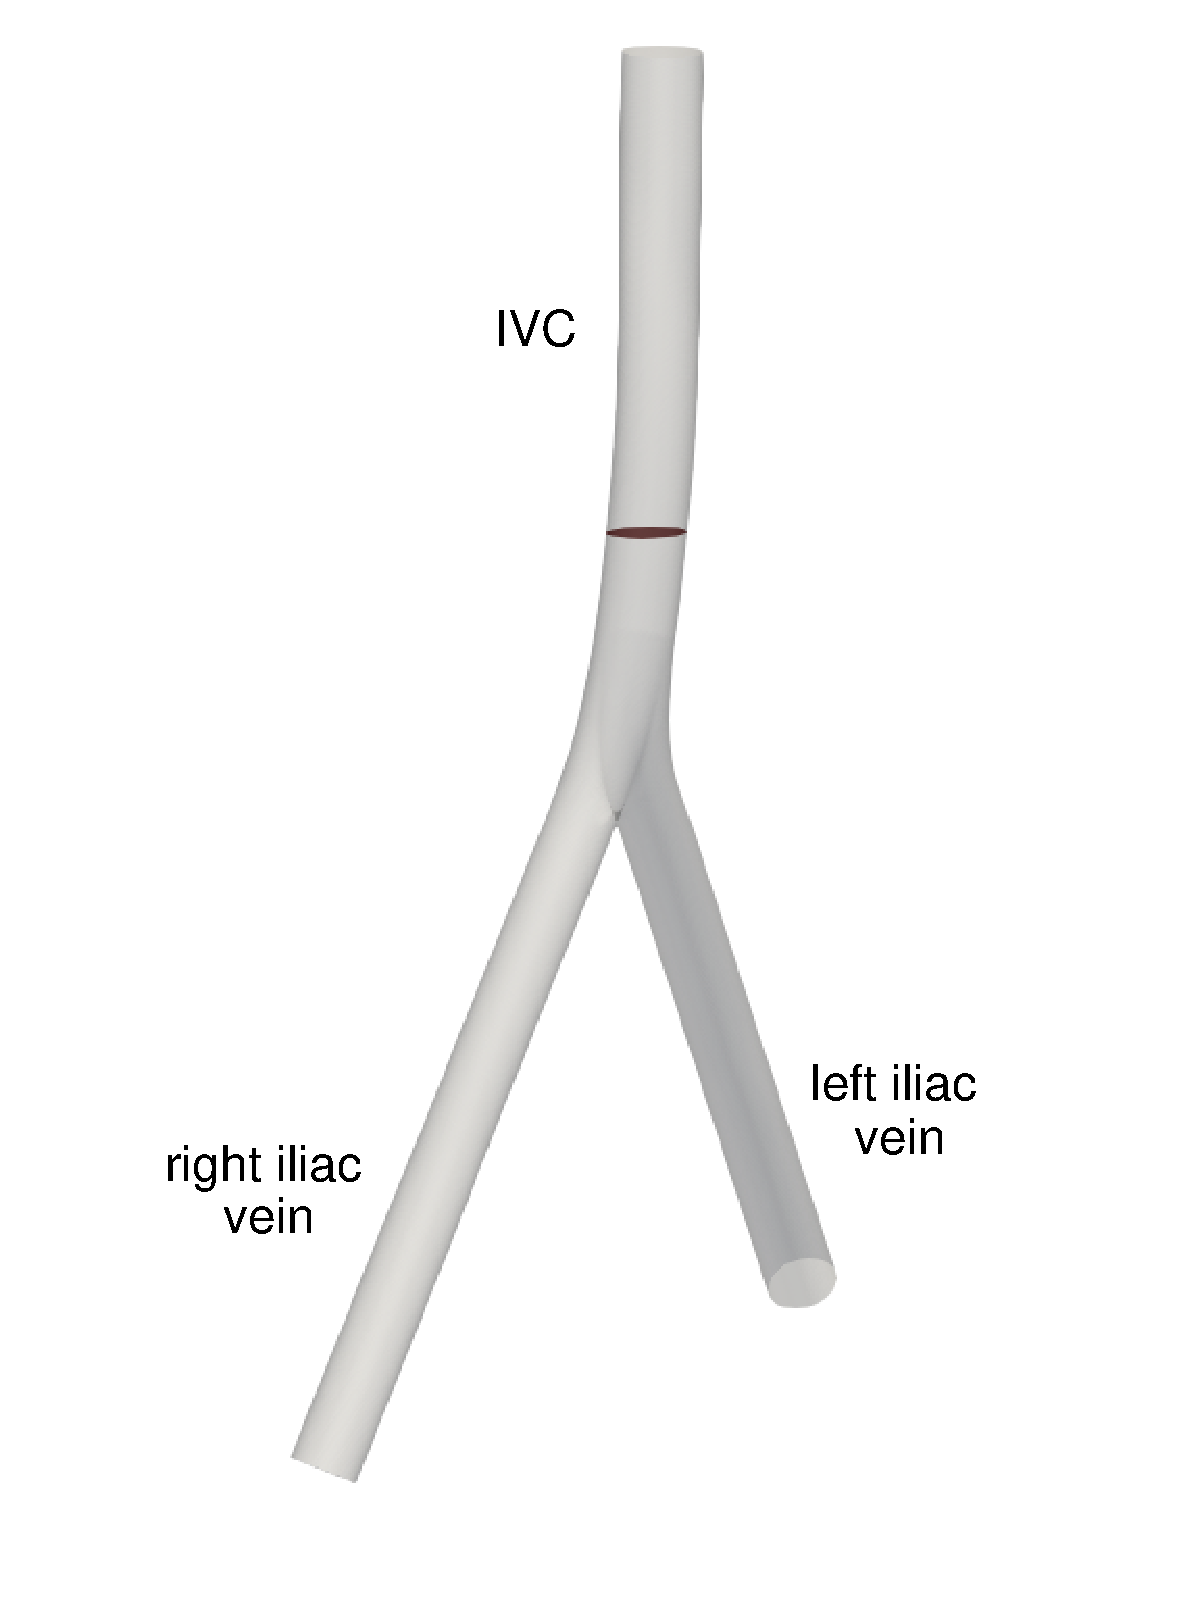
\includegraphics[scale=0.3]{imgs/vena_cava/venacava_plot.eps}
    \caption{The patient-averagved IVC geometry proposed by \cite{gallagher_exp} .}
    \label{fig:IVCgeo}
\end{figure}

\subsubsection*{Grid Convergence Test}

In the grid convergence test, five tetrahedral meshes with different mesh sizes are tested. The mesh sizes are from $0.45$ mm to $2$ mm so that the domain is decomposed into to around $0.87$ million to $37.94$ million tetrahedral elements (Table~\ref{tab:meshsize}). The transverse cross-sections of mesh $2$ and $4$ located at around $10$ cm downstream of the confluence of two iliac veins are shown in the Fig.~\ref{fig:IVCmesh}.

\begin{table}[h]
\caption {Meshes sizes and total element numbers used in the convergence test.} \label{tab:meshsize}
\centering
\begin{tabular}{|c|c|c|}
\hline
Mesh & Number of element ($\times10^6$)& mesh size (mm) \\ \hline
1    & 0.87              & 2.0              \\ \hline
2    & 2.04              & 1.4            \\ \hline
3    & 4.70              & 1.0               \\ \hline
4    & 17.68             & 0.6            \\ \hline
5    & 37.94             & 0.45            \\ \hline
\end{tabular}
\end{table}

\begin{figure}[h]\centering
    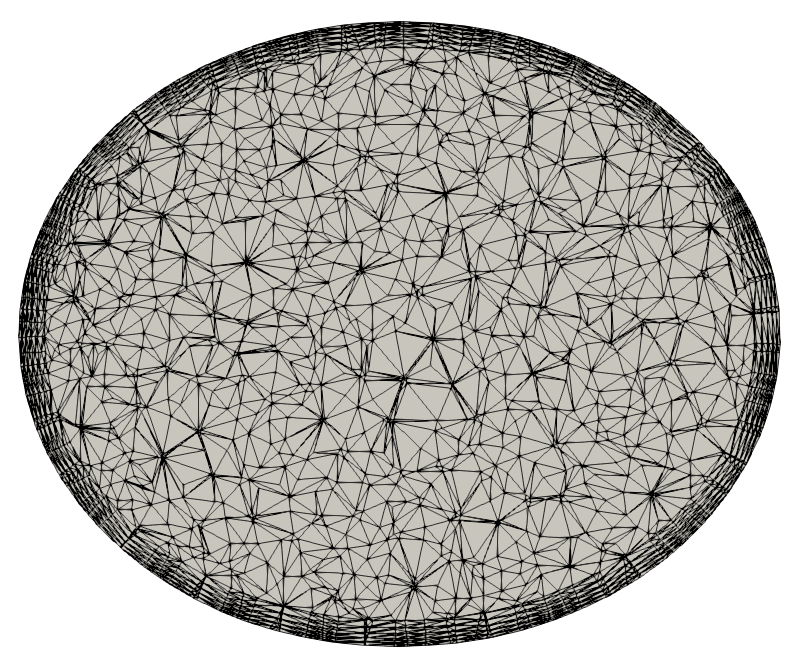
\includegraphics[width=0.5\linewidth]{imgs/vena_cava/mesh2_fixed.png}
    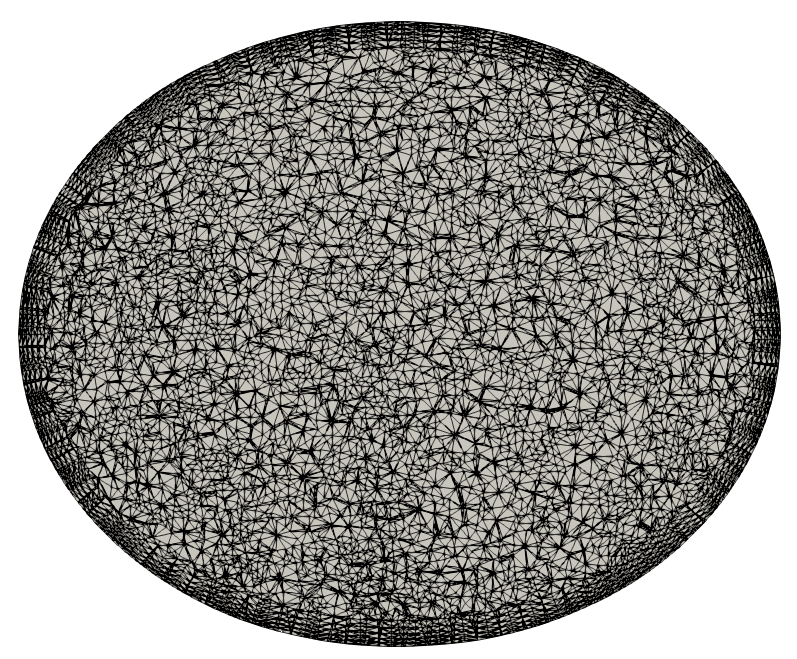
\includegraphics[width=0.5\linewidth]{imgs/vena_cava/mesh4.png}
    \caption{The transverse cross-sectional view of mesh 2 (top) and 4 (bottom) in the grid convergence study. The cross-section is located at 10 cm downstream of the confluence of two iliac veins.}
    \label{fig:IVCmesh}
\end{figure}

The flow simulations with these five meshes are conducted using FEM at exercising condition. The simulation result will be evaluated not only qualitatively with the velocity magnitude field and local normalized helicity field on a transverse cross-sectional plane, but also quantitatively through three scalar quantities: maximum nodal velocity, area-averaged transverse velocity magnitude and volume-averaged helicity intensity. The helicity density $h$, which is defined as the inner product of vorticity and velocity $h=u\cdot\omega$, represents the tendency to have helical flow. The local normalized helicity (LNH) is defined as
\begin{equation}
LNH=\frac{u\cdot\omega}{\left|u\right|\left|\omega\right|},
\label{eq:LNH}
\end{equation}
and the volume-averaged helicity intensity $\overline{HI}$ can be calculated using
\begin{equation}
\overline{HI}=\frac{1}{V}\int_V \left|u\cdot\omega\right| dV.
\label{eq:HI}
\end{equation}
The area-averaged transverse velocity magnitude,
\begin{equation}
\overline{\left|u_{tr}\right|}=\frac{1}{A}\int_A \left|u _\|\right| dA,
\label{eq:utr}
\end{equation}
where $u _\|$ is the velocity component parallel to the surface representing the measure of the secondary flow. The velocity magnitude field, LNH, and $\overline{\left|u_{tr}\right|}$ will be examined on the transverse cross-sectional plane located at $10$ cm downstream of the confluence point in the present study.  

The obtained velocity magnitude field and LNH field with above-mentioned five meshes on the same transverse cross-sectional plane are shown in Fig. \ref{fig:velmag} and \ref{fig:lnh}. It can be observed that the resulting flow velocity fields with different sizes of meshes have the similar patterns, but the some flow details are unresolved with mesh $1$ and $2$. This phenomenon can also be seen in the resulting LNH fields.

\begin{figure*}[htbp]
    \centering
    \begin{minipage}[c][2in][c]{0.4\linewidth}
        \centering
        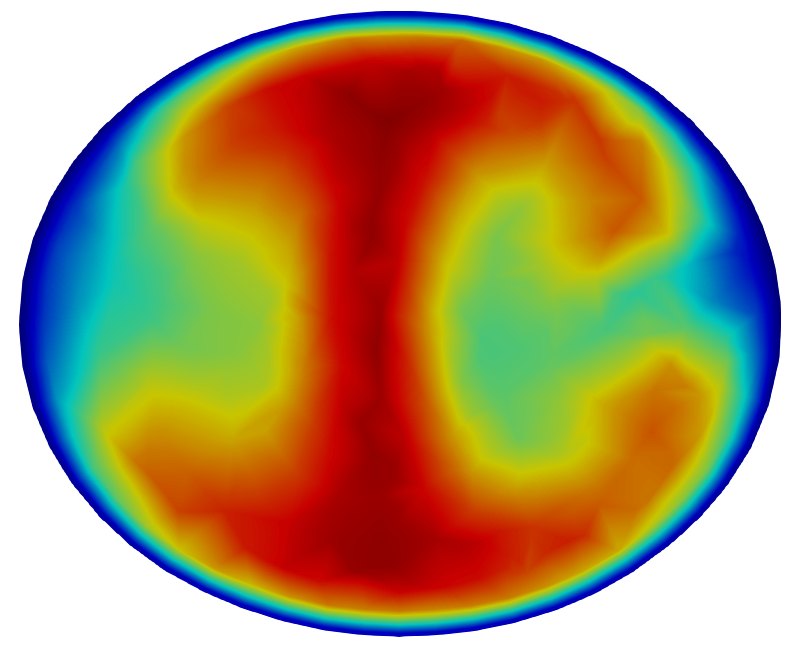
\includegraphics[width=2.3in]{imgs/vena_cava/Umag_mesh1.png}\\
        mesh 1
    \end{minipage}
    \begin{minipage}[c][2in][c]{0.4\linewidth}
        \centering
        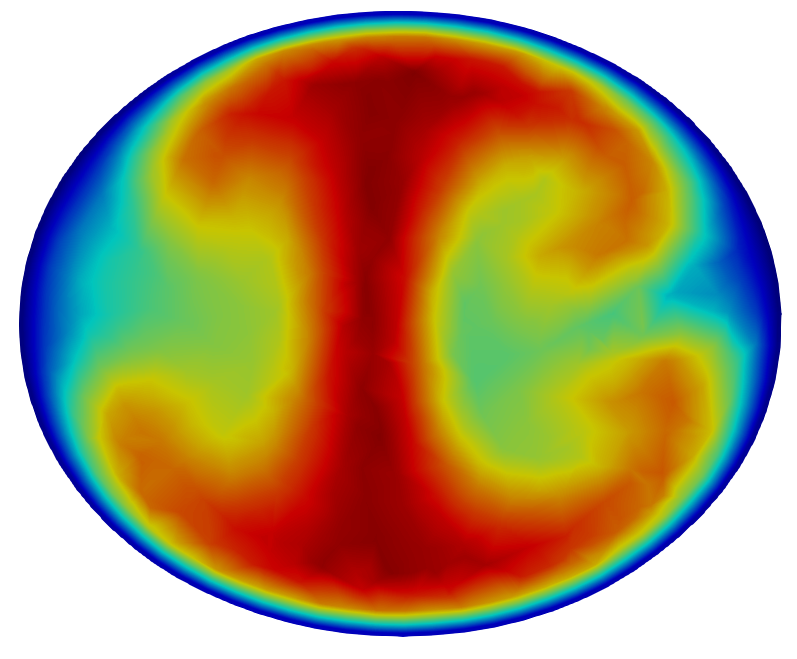
\includegraphics[width=2.3in]{imgs/vena_cava/Umag_mesh2.png}\\
        mesh 2
    \end{minipage}\\[.5\baselineskip]
    \begin{minipage}[c][2in][c]{0.4\linewidth}
        \centering
        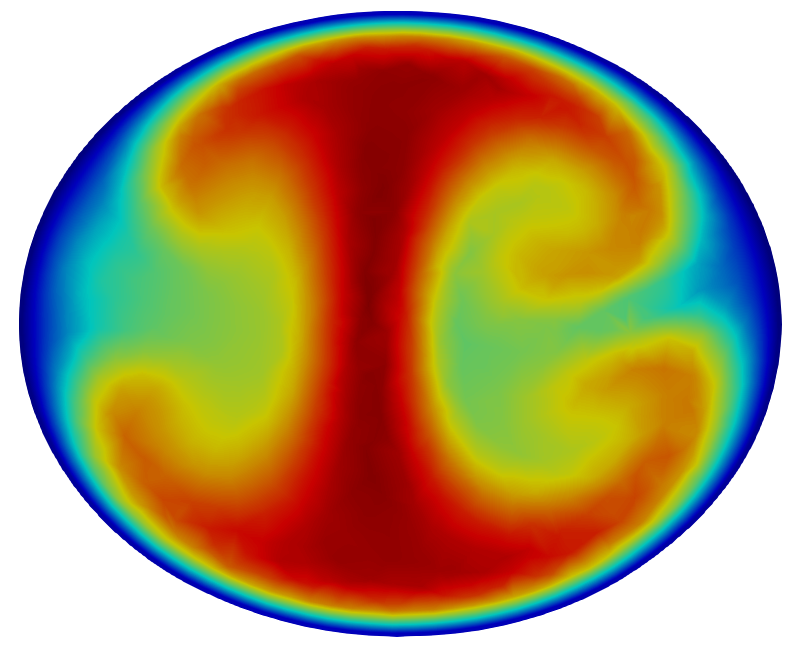
\includegraphics[width=2.3in]{imgs/vena_cava/Umag_mesh3.png}\\
        mesh 3
    \end{minipage}
    \begin{minipage}[c][2in][c]{0.4\linewidth}
        \centering
        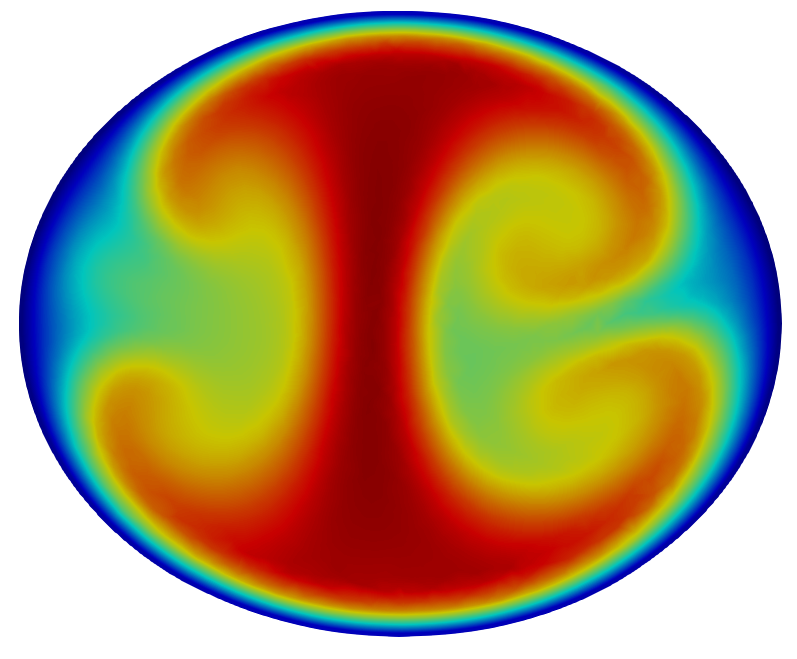
\includegraphics[width=2.3in]{imgs/vena_cava/Umag_mesh4.png}\\
        mesh 4
    \end{minipage}\\[.5\baselineskip]
    \begin{minipage}[c][2in][c]{0.4\linewidth}
        \centering
        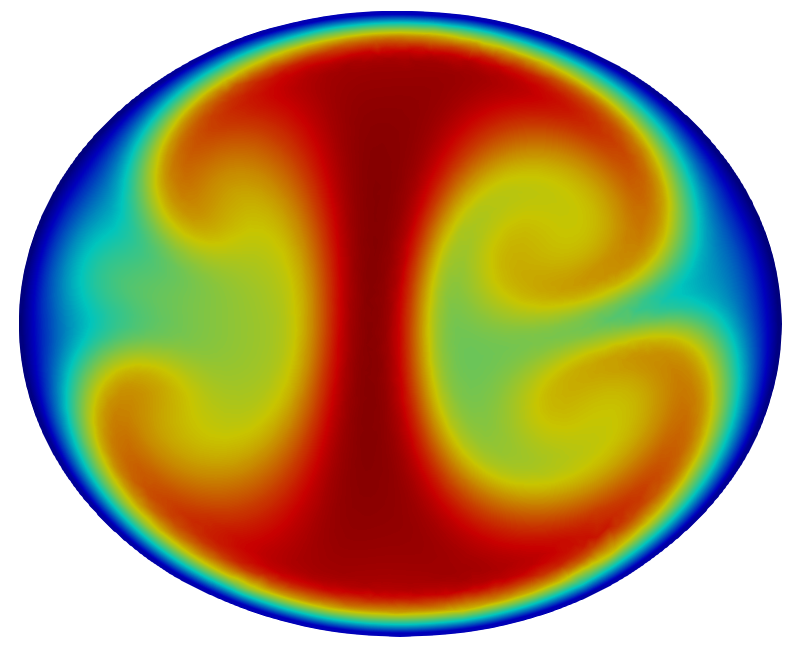
\includegraphics[width=2.3in]{imgs/vena_cava/Umag_mesh5.png}\\
        mesh 5
    \end{minipage}
    \begin{minipage}[c][2in][c]{0.4\linewidth}
        \centering
        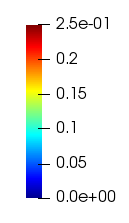
\includegraphics[width=.7in]{imgs/vena_cava/colormap_exercise.png}\\
    \end{minipage}
    \caption{The velocity magnitude fields using different mesh sizes.}
    \label{fig:velmag}
\end{figure*}

\begin{figure*}[htbp]
    \centering
    \begin{minipage}[c][2in][c]{0.4\linewidth}
        \centering
        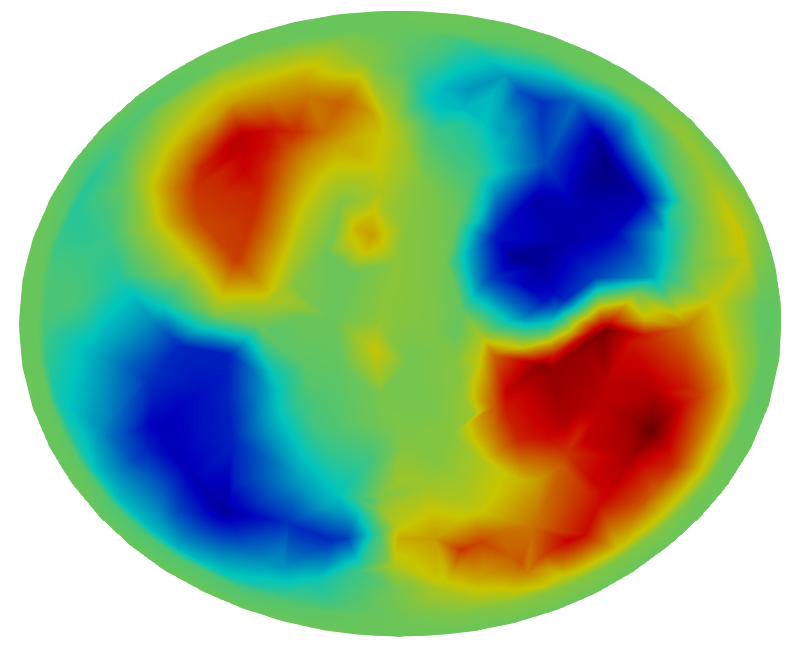
\includegraphics[width=2.3in]{imgs/vena_cava/LNH_mesh1.png}\\
        mesh 1
    \end{minipage}
    \begin{minipage}[c][2in][c]{0.4\linewidth}
        \centering
        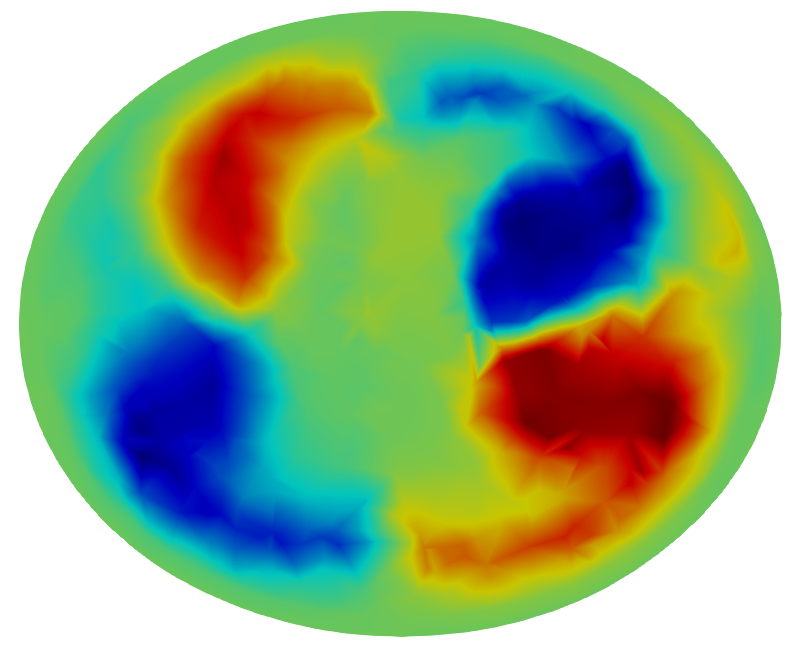
\includegraphics[width=2.3in]{imgs/vena_cava/LNH_mesh2_fixed.png}\\
        mesh 2
    \end{minipage}\\[.5\baselineskip]
    \begin{minipage}[c][2in][c]{0.4\linewidth}
        \centering
        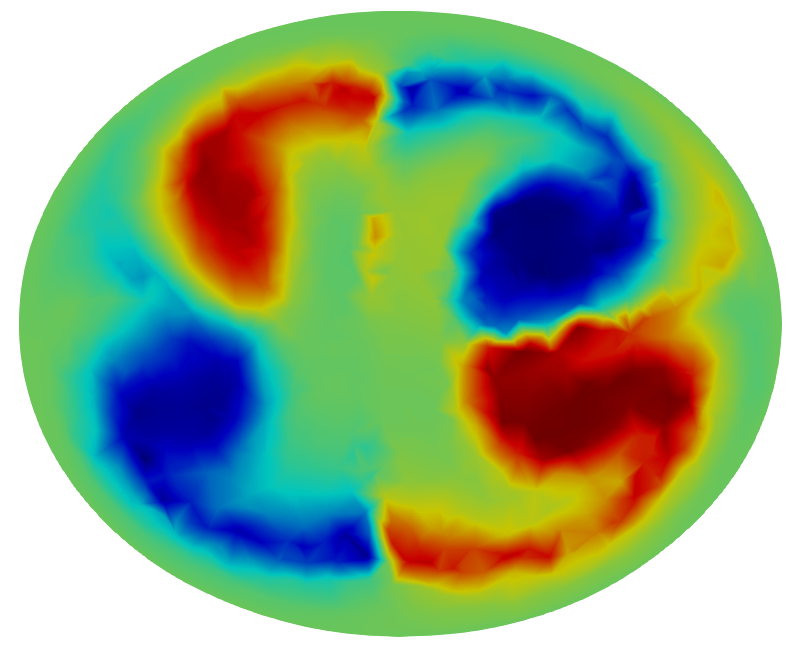
\includegraphics[width=2.3in]{imgs/vena_cava/LNH_mesh3.png}\\
        mesh 3
    \end{minipage}
    \begin{minipage}[c][2in][c]{0.4\linewidth}
        \centering
        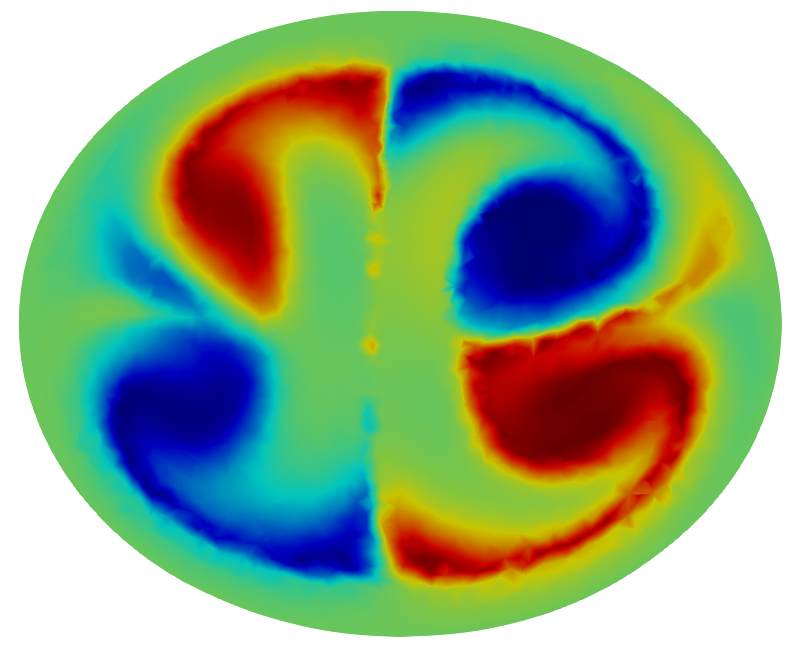
\includegraphics[width=2.3in]{imgs/vena_cava/LNH_mesh4_fixed.png}\\
        mesh 4
    \end{minipage}\\[.5\baselineskip]
    \begin{minipage}[c][2in][c]{0.4\linewidth}
        \centering
        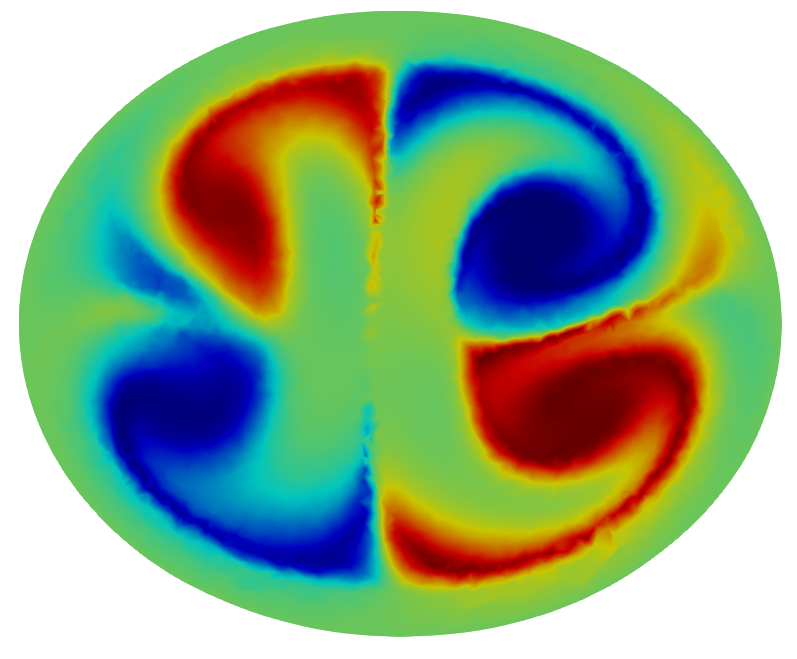
\includegraphics[width=2.3in]{imgs/vena_cava/LNH_mesh5.png}\\
        mesh 5
    \end{minipage}
    \begin{minipage}[c][2in][c]{0.4\linewidth}
        \centering
        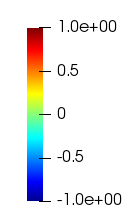
\includegraphics[width=.7in]{imgs/vena_cava/colormap_LNH.png}\\
    \end{minipage}
    \caption{The local normalized helicity (LNH) fields.}
    \label{fig:lnh}
\end{figure*}

The quantitative analysis of the convergence study using maximum nodal velocity, area-averaged transverse velocity magnitude and volume-averaged helicity intensity are tabulated in Table~\ref{tab:convergence}, where $p$ represent the order of convergence.
It can be observed that the transverse velocity and helicity values converge when meshes get finer. But for the maximum nodal velocity, the trend is monotonic except for the result by mesh $1$. This might be because the nodal maximum velocity can be affected by how the domain is decomposed. In the following section, the mesh $2$ and $3$ are chosen in the simulations of IVC flow at resting and exercising conditions.

% choose either one: with  p or not with p
\begin{table*}[]
\centering
\caption {The value of maximum velocity, transverse velocity, Helicity and the corresponding order of convergence $p$.} \label{tab:convergence}
\begin{tabular}{|c|c|c|c|c|c|c|}
\hline
     & \multicolumn{2}{c|}{maximum velocity} & \multicolumn{2}{c|}{transverse velocity} & \multicolumn{2}{c|}{Helicity} \\ \hline
Mesh & $\left |u\right |_{max} $    & p             & $\overline{\left |u_{tr}\right |}$          & p              &   $\overline{HI}$              & p           \\ \hline
1    & 0.2549               &               & 0.0238                 &                & 0.3807         &             \\ \hline
2    & 0.2585               &               & 0.0244                 &                & 0.4132         &             \\ \hline
3    & 0.2567               & 2.36       & 0.0247                 & 2.40          & 0.4331         & 1.63        \\ \hline
4    & 0.2541               & 0.31       & 0.02497                 & 2.24          & 0.4498         & 1.84        \\ \hline
5    & 0.2534	          &  2.16      & 0.02502                 & 2.88          & 0.4536         &  2.54        \\ \hline
\end{tabular}
\end{table*}
% 
\iffalse
\begin{table}[h]
\caption {} \label{tab:convergence}
\centering
\begin{tabular}{|c|c|c|c|}
\hline
Mesh & $u_{max}$ & Transverse velocity &  Helicity       \\ \hline
1    & 0.25486           & 0.02380        & 0.38067 \\ \hline
2    & 0.25846           & 0.02443        & 0.41316 \\ \hline
3    & 0.25666           & 0.02474        & 0.43313 \\ \hline
4    & 0.25409           & 0.02497        & 0.44978 \\ \hline
5     & 0.25341	      & 0.02502        & 0.45361         \\ \hline
\end{tabular}
\end{table}
\fi
%------------------------------------

\subsubsection*{Comparison with Experimental Results}

The velocity fields predicted by FEM and PFEM-2 solvers will be compared quantitatively with PIV experimental result by \cite{gallagher_exp} on a selected sagittal plane and a coronal plane as illustrated in Fig.~\ref{fig:IVCPIV} at two flow conditions. The FEM and PFEM-2 solvers use the same mesh under the same flow condition. The experimental and simulation results of the in-plane 2D velocity magnitudes in the sagittal and coronal planes at resting and exercising conditions are shown in the Fig \ref{fig:rest} and \ref{fig:exercise}. It shows that the results by FEM and PFEM-2 solvers both match qualitatively with the PIV results. 

\begin{figure}[htbp]
    \centering
    \begin{minipage}[c][8cm][c]{0.15\textwidth}
    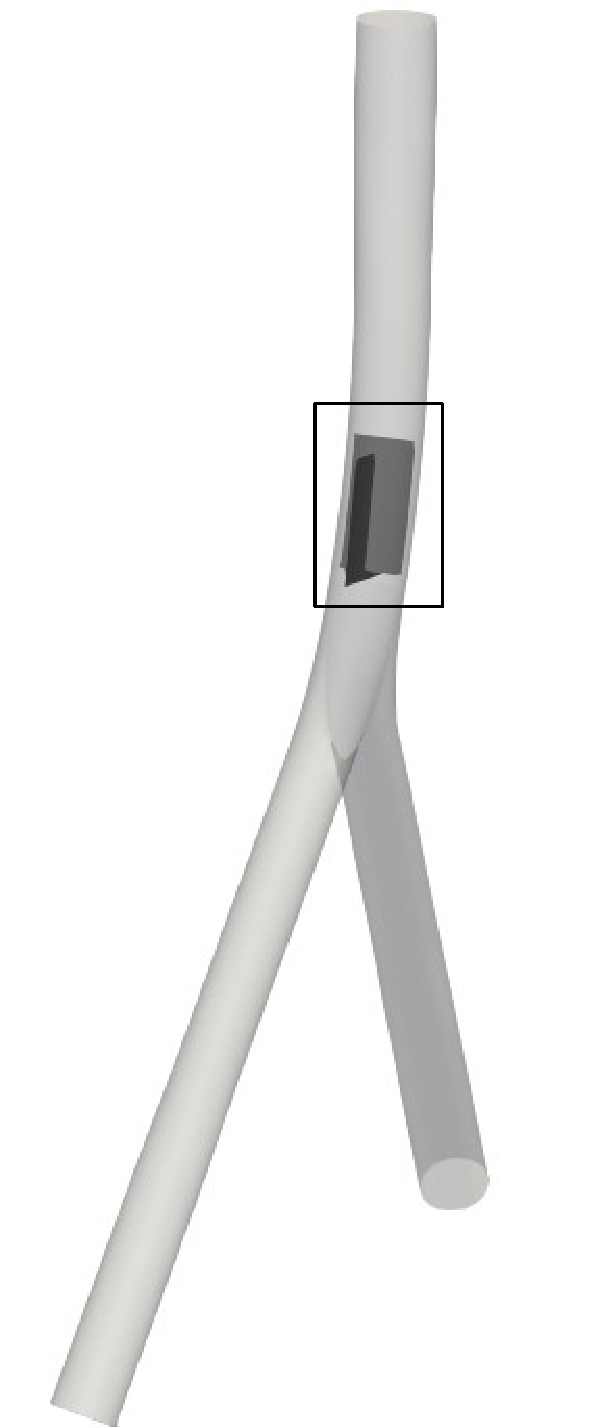
\includegraphics[scale=0.28]{imgs/vena_cava/venacava_piv1.pdf}
    \end{minipage}
    \begin{minipage}[c][8cm][c]{0.2\textwidth} 
    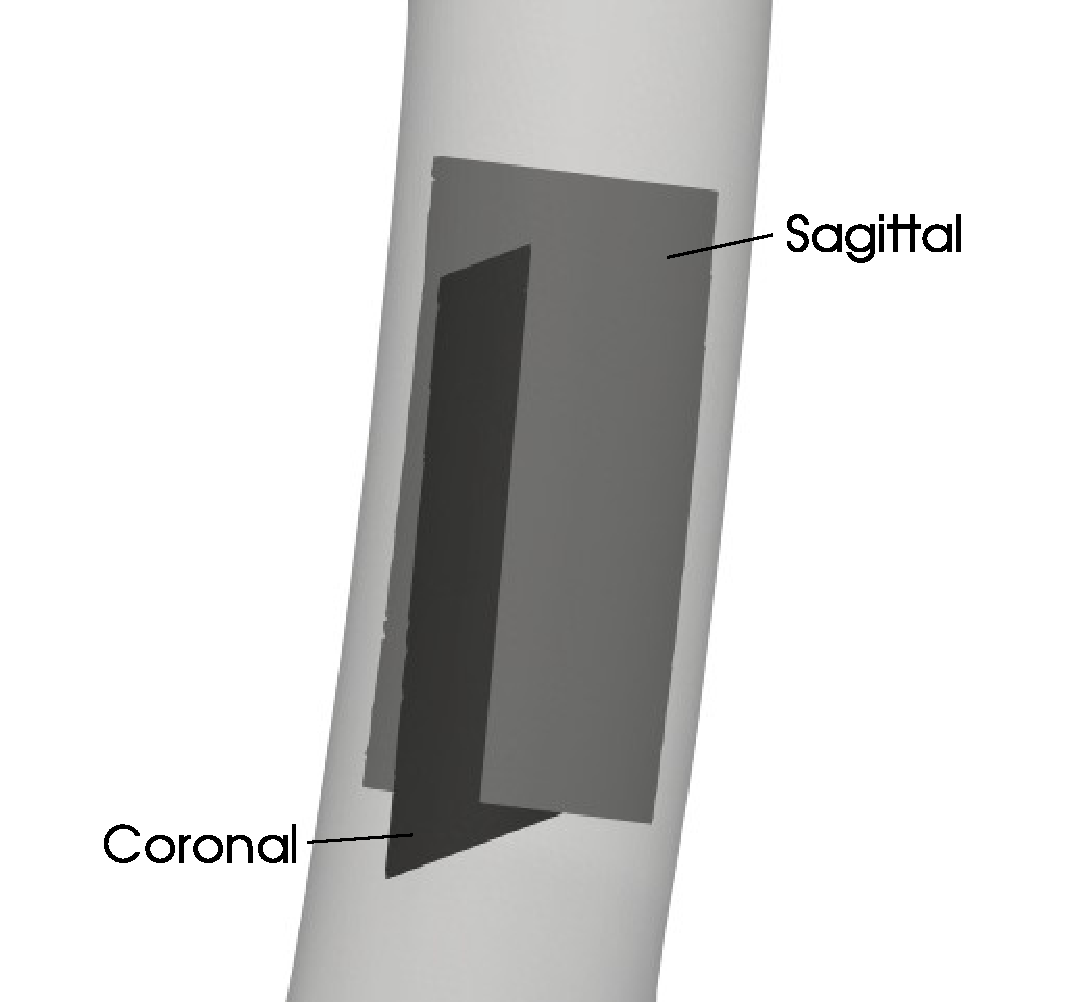
\includegraphics[scale=0.25]{imgs/vena_cava/venacava_piv3.pdf}
    \end{minipage} 
    \caption{The sagittal and coronal planes where the velocity field are measured in experiment \cite{gallagher_exp}.}
    \label{fig:IVCPIV}
\end{figure}

\begin{figure*}\centering
\begin{minipage}[c][10cm][c]{0.25\textwidth}
\centering
\vspace*{\fill}
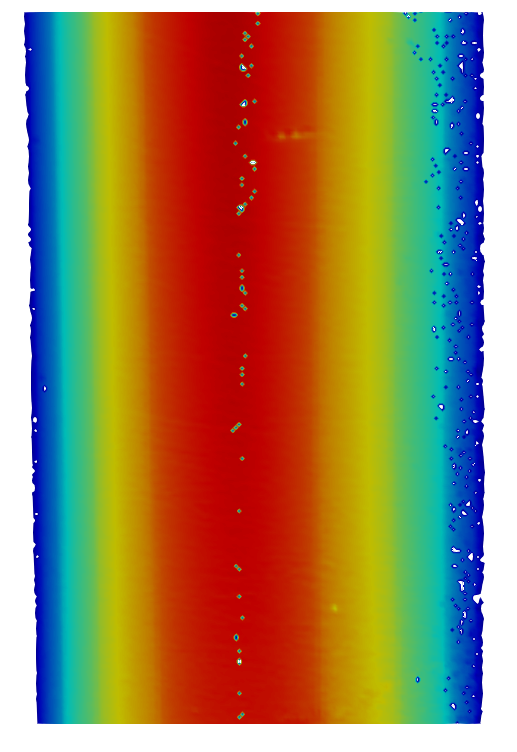
\includegraphics[height=4cm]{imgs/vena_cava/PIV_coronal_rest.png}
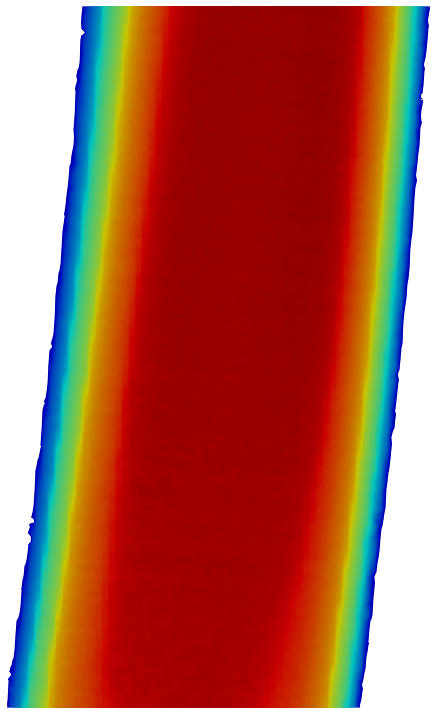
\includegraphics[height=5cm]{imgs/vena_cava/PIV_sagittal_rest.png}
\\PIV
\end{minipage}
\begin{minipage}[c][10cm][c]{0.25\textwidth}
\centering
\vspace*{\fill}
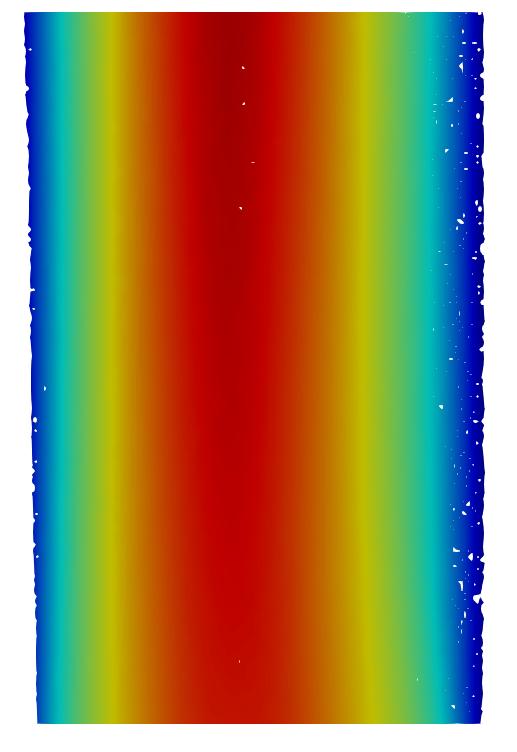
\includegraphics[height=4cm]{imgs/vena_cava/FEM_coronal_rest.png}
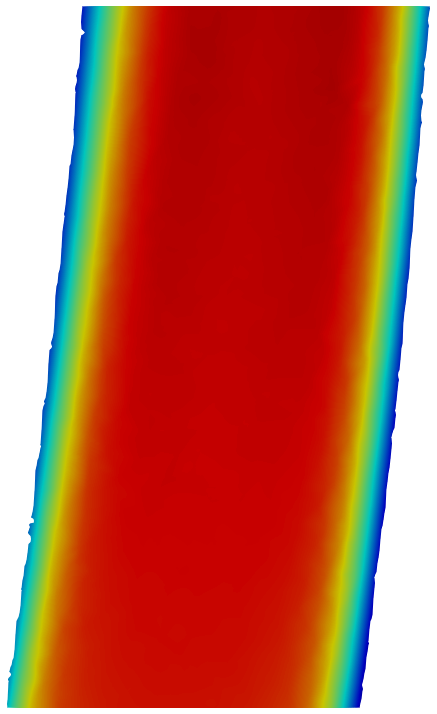
\includegraphics[height=5cm]{imgs/vena_cava/FEM_sagittal_rest.png}
\\FEM
\end{minipage}
\begin{minipage}[c][10cm][c]{0.25\textwidth}
\centering
\vspace*{\fill}
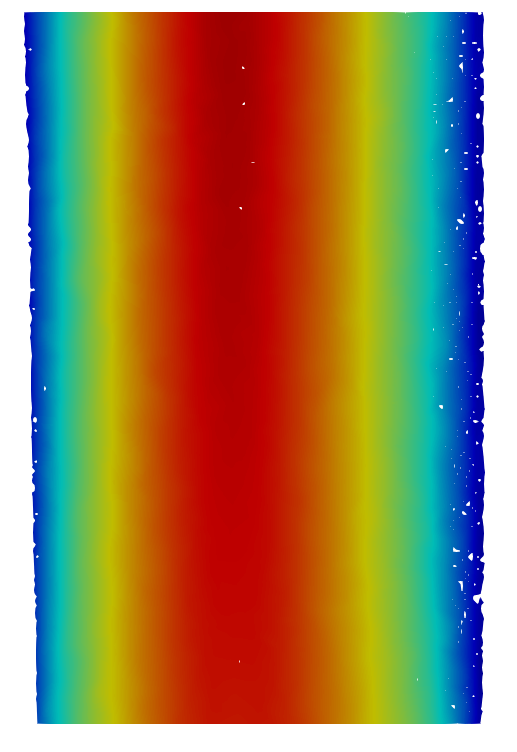
\includegraphics[height=4cm]{imgs/vena_cava/PFEM_coronal_rest.png}
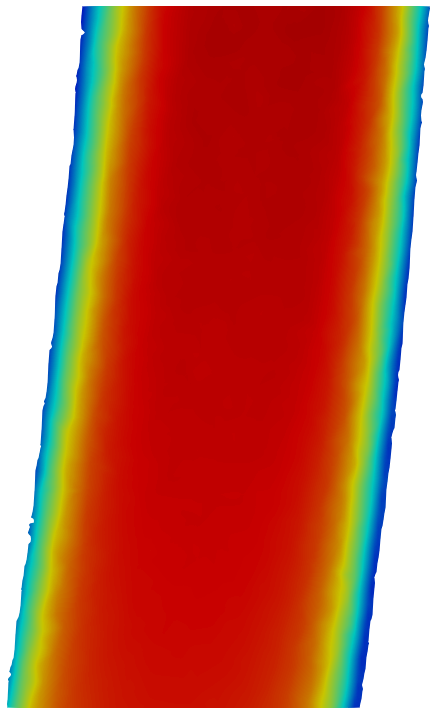
\includegraphics[height=5cm]{imgs/vena_cava/PFEM_sagittal_rest.png}
\\PFEM-2
\end{minipage}
\begin{minipage}[c][10cm][t]{0.1\textwidth}
\vspace*{\fill}
\centering
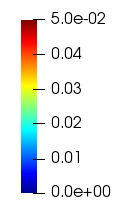
\includegraphics[height=3cm]{imgs/vena_cava/colormap_rest.png}
\\
\end{minipage}
\caption{The in-plane 2D velocity magnitude in coronal (top) and sagittal (bottom) planes of PIV, FEM and PFEM-2 results at resting condition}
\label{fig:rest}
\end{figure*}

\begin{figure*}\centering
\begin{minipage}[c][10cm][c]{0.25\textwidth}
\centering
\vspace*{\fill}
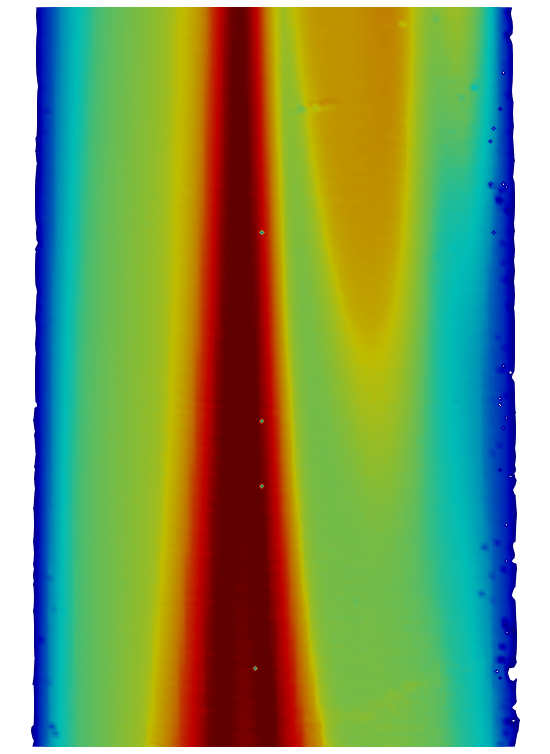
\includegraphics[height=4cm]{imgs/vena_cava/PIV_coronal_exercise.png}
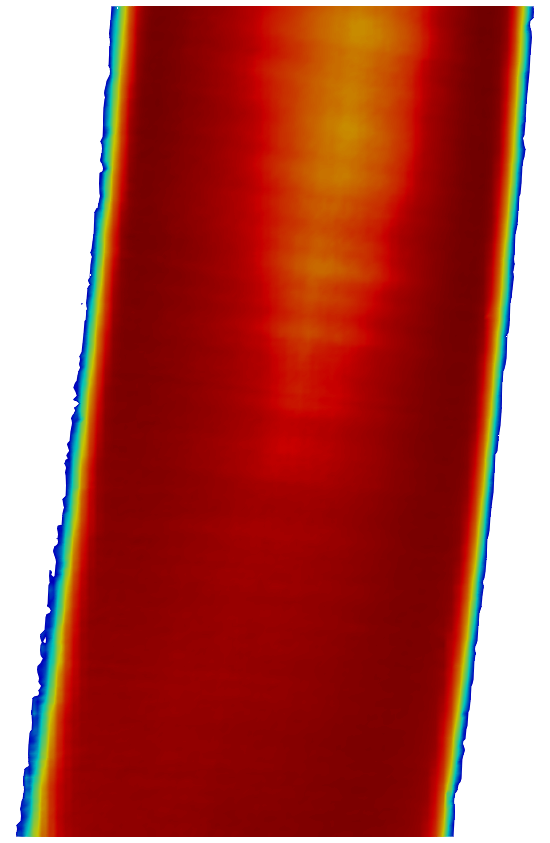
\includegraphics[height=5cm]{imgs/vena_cava/PIV_sagittal_exercise.png}
\\PIV
\end{minipage}
\begin{minipage}[c][10cm][c]{0.25\textwidth}
\centering
\vspace*{\fill}
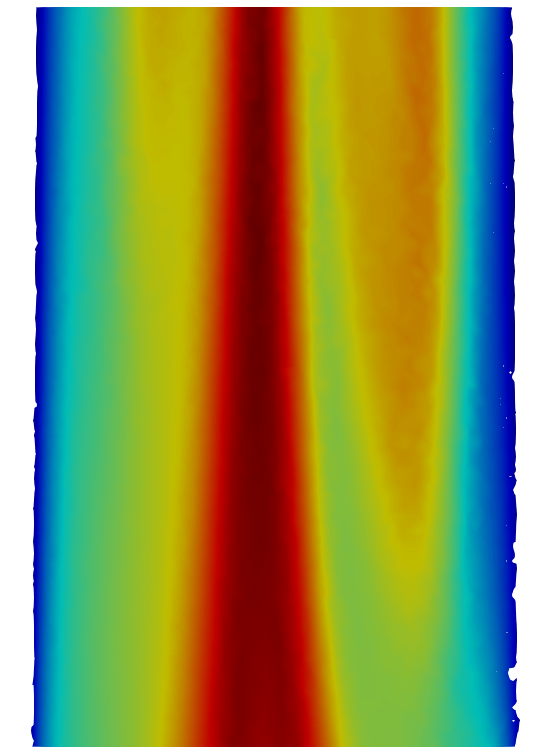
\includegraphics[height=4cm]{imgs/vena_cava/FEM_coronal_exercise.png}
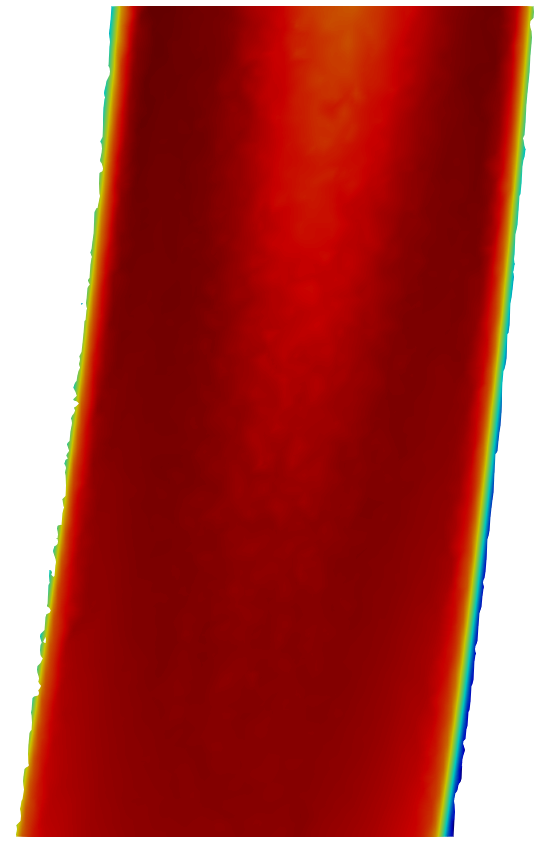
\includegraphics[height=5cm]{imgs/vena_cava/FEM_sagittal_exercise.png}
\\FEM
\end{minipage}
\begin{minipage}[c][10cm][c]{0.25\textwidth}
\centering
\vspace*{\fill}
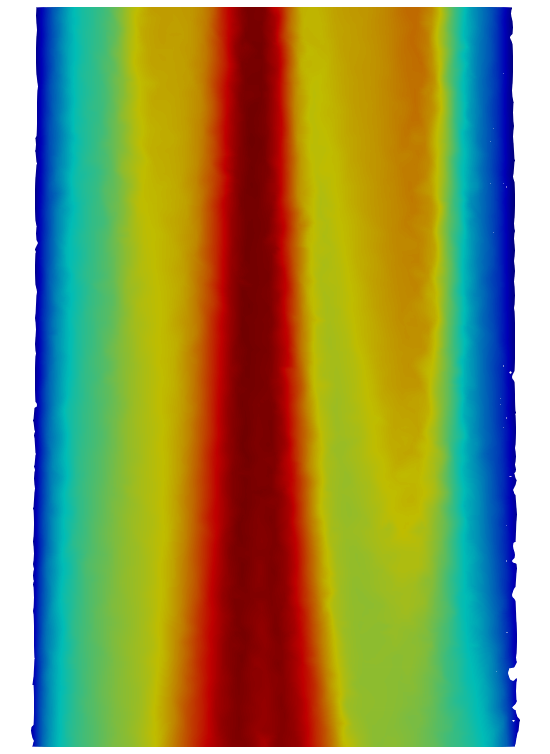
\includegraphics[height=4cm]{imgs/vena_cava/PFEM_coronal_exercise.png}
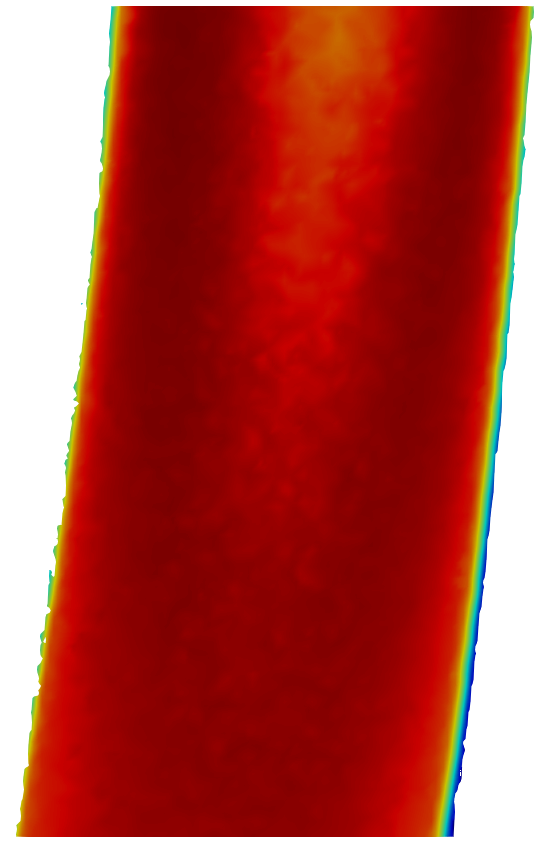
\includegraphics[height=5cm]{imgs/vena_cava/PFEM_sagittal_exercise.png}
\\PFEM-2
\end{minipage}
\begin{minipage}[c][10cm][t]{0.1\textwidth}
\vspace*{\fill}
\centering
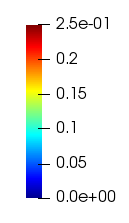
\includegraphics[height=3cm]{imgs/vena_cava/colormap_exercise.png}
\\
\end{minipage}
\caption{The in-plane 2D velocity magnitude in coronal (top) and sagittal (bottom) planes of PIV, FEM and PFEM-2 results at resting condition}
\label{fig:exercise}
\end{figure*}

To do quantitative comparison with experiments, the numerically obtained nodal velocities are firstly sampled on to the PIV data points. The magnitude of 2D plane velocity is then calculated on each data points. The global relative error, $E$, can be obtained by averaging the relative error between numerical and experimental result on all the points. Table \ref{tab:rest} and \ref{tab:exercise} shows the global relative error at different flow conditions with FEM, PFEM-2 solvers as well as the numerical analysis reported in \cite{craven_cfd}. The global relative error is around $5$ to $6$\% at resting condition and $6$ to $11$\% at exercising condition. The obtained numerical results have a good agreement with the experimental data. For both conditions, the FEM and PFEM-2 results have similar amount of global relative error with \cite{craven_cfd}. It is worth noting that the mesh sizes used here ($1.4$ mm for resting and $1$ mm for exercising) are coarser than the mesh size ($0.276$ mm) used in \cite{craven_cfd}. Also, the PFEM-2 has nearly the same error compared with FEM at resting condition, and even less error in the coronal plane at exercising condition.

\begin{table}[h!]
\caption {Global relative error (\%) between numerical and PIV data at resting condition.} \label{tab:rest}
\centering
\begin{tabular}{|c|c|c|}
\hline
       & Coronal & Sagittal \\ \hline
\cite{craven_cfd}  & 3.07    & 6.77     \\ \hline
FEM    & 4.83    & 6.62     \\ \hline
PFEM-2 & 4.79    & 6.65     \\ \hline
\end{tabular}
\end{table}

\begin{table}[h!]
\caption {Global relative error (\%) between numerical and PIV data at exercising condition.} \label{tab:exercise}
\centering
\begin{tabular}{|c|c|c|}
\hline
       & Coronal & Sagittal \\ \hline
\cite{craven_cfd}  & 10.98	&5.56 \\ \hline
FEM    &  11.28    &  5.93  \\ \hline
PFEM-2 &  10.44   &  6.10     \\ \hline
\end{tabular}
\end{table}
